\documentclass[a4paper,12pt]{article}
\usepackage[T1]{fontenc}
\usepackage[latin9]{inputenc}
\usepackage{listings}
\usepackage{amsmath}
\usepackage{mathtools}
\usepackage{hyperref}
\usepackage{mathpazo}
\usepackage{wasysym}
\usepackage{graphicx}
\usepackage[colorinlistoftodos]{todonotes}
\usepackage{natbib} 
\usepackage{geometry}
\usepackage{tikz}
\geometry{verbose,tmargin=2.5cm,bmargin=2.5cm,lmargin=3cm,rmargin=3cm}

\DeclarePairedDelimiter{\ceil}{\lceil}{\rceil}
\DeclarePairedDelimiter{\floor}{\lfloor}{\rfloor}
\newcommand{\ord}{\operatorname{ord}}

\newcommand*\circled[1]{\tikz[baseline=(char.base)]{
            \node[shape=circle,draw,inner sep=2pt] (char) {#1};}}

\begin{document}

\title{I/O-algorithms\\Project 3}

\author{Lasse Espeholt - 20093223\\
Kasper Nielsen - 20091182\\}

\maketitle

\pagebreak{}\tableofcontents{}\pagebreak{}

\section{Sorting}
In this exercise an I/O-efficient algorithm for removing duplicates in a multiset of $N$ elements is analyzed. As given in the hint in the exercise, the algorithm is based on merge-sort, where duplicates are removed as soon as they are found in the merge step.

The algorithm will be analyzed by giving an upper bound on the number of times an element is scanned during an execution of the algorithm. For illustration purposes consider Figure~\ref{fig:sorting:mergetree}. Since duplicates are removed as soon as they are found, no node in the merge tree can contain duplicates (the leaves are found by sorting the elements in internal memory and removing duplicates).

\begin{figure}[h!]
  \centering
  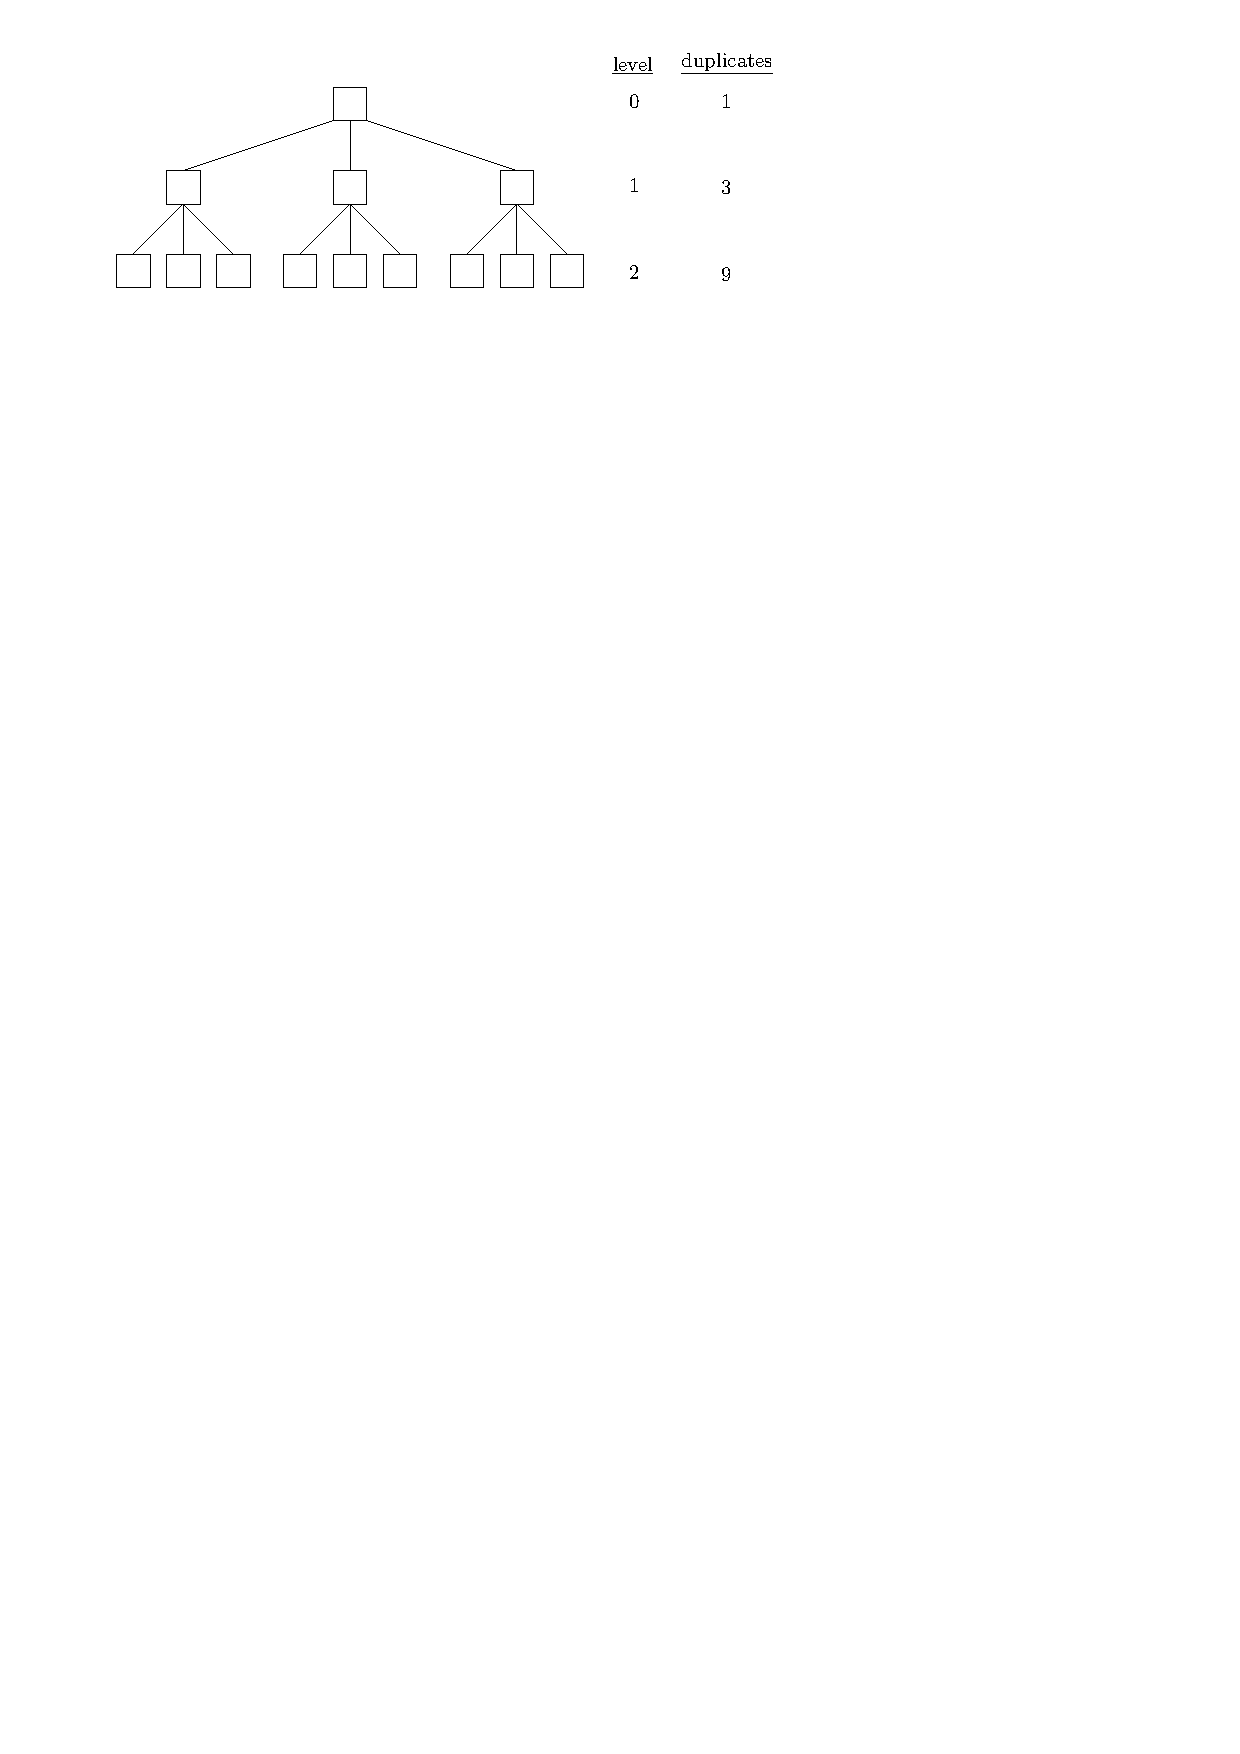
\includegraphics[width=0.8\textwidth]{images/mergetree}
  \caption{Example merge tree of height $3$ with fanout $d = 3$. Illustrates how many duplicates there can be on every level of the merge tree.}
  \label{fig:sorting:mergetree}
\end{figure}

Therefore for a given level $l$ in the merge tree of fanout $d$ and height $H$, at most $d^l$ duplicates remain. Furthermore, there is at most $N_i$ duplicates of a given element $i$. Therefore, the total number of duplicates remaining on level $i$ is less than $\min\{d^l, N_i\}$. Summing the contribution from all levels of the tree gives an upper bound on the number of times a given element is scanned. This can again be summed over all different elements, giving the following bound on the total number of element scans
\[
  \sum_{i=1}^K \sum_{l = 0}^H \min\{N_i, d^l\} .
\]
It is noticed that $N_i \leq d^l \iff \log_d{N_i} \leq l$. Therefore, if $H_i := \floor{\log_d{N_i}}$, then
\[
  \sum_{i=1}^K \sum_{l = 0}^H \min\{N_i, d^l\} =
    \sum_{i=1}^K \left( \sum_{l=0}^{H_i} d^l + \sum_{l = H_i + 1}^H N_i \right) =
    \underbrace{\sum_{i=1}^K \sum_{l=0}^{H_i} d^l}_{\circled{1}} + \underbrace{\sum_{i=1}^K \sum_{l = H_i + 1}^H N_i}_{\circled{2}}.
\]
An upper bound is given on \circled{1} and \circled{2}:
\begin{description}
\item[\circled{1}] Notice that\todo{Should we show this?}
  \begin{align*}
    \sum_{l=0}^{H_i} d^l = \frac{d^{H_i + 1} - 1}{d - 1} = \frac{d d^{\floor{\log_d{N_i}}} - 1}{d - 1} \leq \frac{d}{d - 1} N_i .
  \end{align*}
  When summing over all elements, it is found that
  \[
    \circled{1} \leq \sum_{i=1}^K \frac{d}{d - 1} N_i = \frac{d}{d - 1} N.
  \]
  By the tall cache assumption $d = \frac{M}{B} \geq B \geq 2$ (otherwise it is an internal memory algorithm). Therefore $\frac{d}{d - 1} \leq 2$, hence $\circled{1} = O(N)$.

\item[\circled{2}] For this bound, notice that
  \begin{align*}
    \sum_{l = H_i + 1}^{H} N_i &= \left( H - (H_i + 1) \right) N_i
      = \left( \log_d{\frac{N}{M}} - (\floor{\log_d{N_i}} + 1) \right) N_i \\
      &\leq \left( \log_d{\frac{N}{M}} - \log_d{N_i} \right) N_i
      = N_i \log_d{\frac{N}{M}} - N_i \log_d{N_i}.
  \end{align*}
  By summing over all elements, it is found that
  \[
    \circled{2} \leq \sum_{i=1}^K N_i \log_{\frac{M}{B}}{\frac{N}{M}} - N_i \log_{\frac{M}{B}}{N_i}
      = O\left( N \log_{\frac{M}{B}}{\frac{N}{B}} - \sum_{i = 1}^K N_i \log_{\frac{M}{B}}{N_i} \right).
  \]
\end{description}
Combining theses two bounds, it is found that at most
\[
  \sum_{i=1}^K \sum_{l = 0}^H \min\{N_i, d^l\} = O(N) + O\left( N \log_{\frac{M}{B}}{\frac{N}{B}} - \sum_{i = 1}^K N_i \log_{\frac{M}{B}}{N_i} \right)
\]
elements are scanned during the algorithm. The algorithm always scans elements in blocks, however some of the blocks could be non-full due to the duplicate removal. However, this can only happen once for every node in the merge tree, which is asymptotically bounded by the number of leaves ($\frac{N}{M} \leq \frac{N}{B}$). Therefore this cost and the cost of the first input scans are bounded by $O(\frac{N}{B}))$, whereby the total number of I/Os is bounded by
\begin{align*}
  O\left( \max\left\{ \frac{N}{B}, \frac{N \log_{\frac{M}{B}}{\frac{N}{B}} - \sum_{i = 1}^K N_i \log_{\frac{M}{B}}{N_i}}{B} \right\} \right) \\
    = O\left( \max\left\{ \frac{N}{B}, \frac{N}{B} \log_{\frac{M}{B}}{\frac{N}{B}} - \sum_{i=1}^K \frac{N_i}{B} \log_{\frac{M}{B}}{N_i} \right\} \right).
\end{align*}

\pagebreak
\section{Searching}
This exercise describes how an external linear space data structure can be designed, which maintain a set of intervals such that the number of intervals containing a given point can be reported in $O(\log_B^2 N)$ I/Os. Also the structure should have support for inserts and deletes in amortized $O(\log_B^2 N)$ I/Os.

The problem is very closely related to the one solved by the external interval tree -- instead of reporting the stabbed intervals, they should be counted. However, this means that some of the complexity of the data structure can not be hidden behind the output complexity. In order to circumvent this problem, the following modifications are made to the external interval tree:
\begin{itemize}
  \item The slab lists associated to a node are stored as a weight balanced B-tree.
  \item A counter is associated to all multislab lists, maintaining the number of intervals in the multislab. These counters also stores the counts for the intervals put in the underflow structure.

\iffalse
  \item In addition to the underflow structure, a counting underflow structure is maintained. The static structure for answering interval queries used in the underflow structure is modified such that it can answer counting stabbing queries in time $O(\log_B N)$ I/Os. This is done by sweeping the intervals from left to right, and maintain a counter of the number of currently active intervals. For all start or endpoints of intervals, the current number of active intervals is inserted into a B-tree. Thereby a counting stabbing query can be answered by searching down the B-tree. Clearly this structure uses linear space and can be constructed in $O(\frac{N}{B} \log_{\frac{M}{B}}{\frac{N}{B}})$ I/Os.

  Notice that instead of storing the counting underflow structure, it could be omitted and then simply store the counts in the counters for the multislabs. However, we have chosen not to do this in order to have a more clear correspondence with the external interval tree.
\fi
\end{itemize}
Since the original external interval tree uses linear space, the structure with the above modifications still uses linear space.

Queries are answered by walking down the base tree based on the query point. When processing a node in the tree the counts for the multislab lists are loaded using $O(1)$ I/O, and the relevant interval counts are summed. Then the associated structure to the node is queried as described below using $O(\log_B N)$ I/Os. Then the query is called recursively in the base tree, leading to a query complexity of $O(log_B^2 N)$ I/Os.

When querying the associated data-structures, it should be counted how many elements are located to the left (right) of a given point. In the original external interval tree, this was done by scanning the elements, and then charging the cost to the output size. However, this is not possible when counting. Instead, a query is answered by walking down the tree according to the query points, and then count the number of elements in the sub-trees to the left (right) by using their weights.

Figure~\ref{fig:searching:query} illustrates the query process for counting the number of intervals in the right slab lists. The querying process is started in the root, and is then moving down the tree. Every internal node stores the weights of all the children, which can be loaded using $O(1)$ I/Os, and can also be updated without a problem during insertion/deletion. In order to find the number of intervals to the left of a given point, the children of $v$ located to the left of the child $v'$ containing the query point is summed up, and a recursive call is made on $v'$.
\begin{figure}[h!]
  \centering
  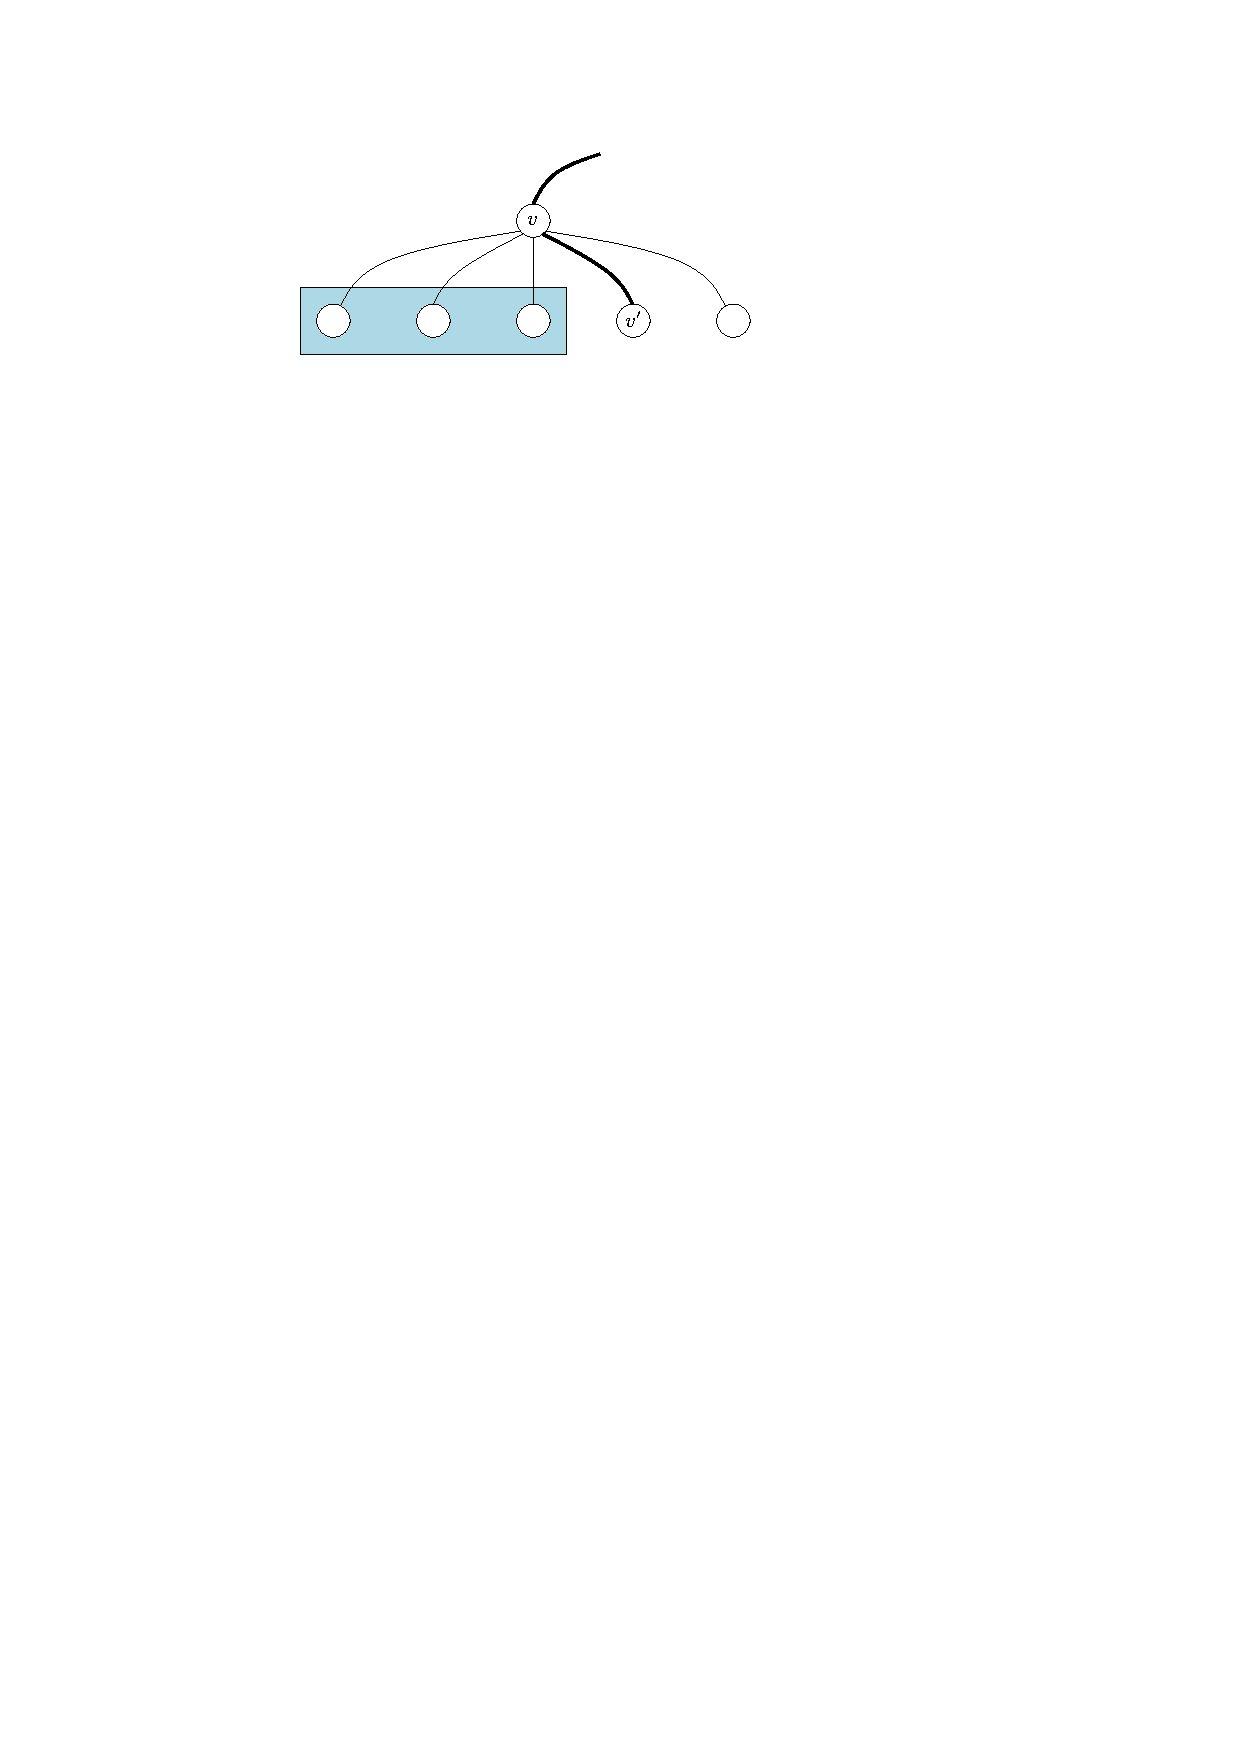
\includegraphics[width=0.6\textwidth]{images/query}
  \caption{Answering a query in a right slab list structure. The weights of the leafs to the left of $v'$ is summed up to get the number of intervals to the left of the query point.}
  \label{fig:searching:query}
\end{figure}
This procedure $O(1)$ I/Os at every node and since the tree is balanced, contributes a total of $O(\log_B N)$ I/Os.

The insertion / deletion process is almost the same as for the external interval tree\footnote{We assume the version without global rebuilding when doing deletions.}. The only difference is that the counters for the multislabs needs to be updated, but this can easily be done when updating the elements inside each multislab. Using the same analysis as in the lecture notes, the complexity for doing inserts and deletes is $O(\log_B N)$ I/Os amortized.

\pagebreak
\section{Distribution sweeping}

\textbf{Problem:} Given $N$ rectangles in the plane, compute the measure (area) of their union.
\\
\\We solved the problem with the following algorithm which is visualized in figure~\ref{fig:segments}.

\subsection{Algorithm}

\begin{enumerate}
\item \label{enu:segments} Construct 4 segments for each rectangle consisting of an 'overlap' attribute initialized to 0 and an associated list of rectangles that has a corner point at the segment. Initially the list only contains the rectangle the segment is constructed from. In total $4N$ segments are constructed. These segments are shown in figure~\ref{segment2}. The 'overlap' attribute describes how large a part is overlapped by rectangles from the segment to the next segment (the one with the next $y$ value).
\item \label{enu:sorting} Sort segments by $x$ value, then by $y$. When sorting, all segments are points, therefore the $x$ value is well defined. The sorting can be done using two external mergesorts. A \emph{strip} is created for all different values of $x$. A strip contains a $x$-coordinate, a 'width' attribute and a list of segments. Initially a strip has a width of 0 and all the segments that has the given $x$ value.
\item \label{enum:combine} Combine $d$ strips until only one strip remains by (shown in figure~\ref{segment3}, \ref{segment4} and \ref{segment5})
    \begin{enumerate}
        \item Iterating through all $d$ strips by $y$ value. Each iteration combines between 1 and $d$ segments. I.e. there might only be one segment with the next lowest $y$ value or there might be a segment in all $d$ strips with the next lowest $y$.
        \item Two arrays $E$ and $W$ are updated while iterating the strips. $E$ contains $d$ counts where $E_i>0$ means that some rectangle is covering the horizontal area strip $i$ covers. $W$ contains $d-1$ counts where $W_i>0$ means that some rectangle is covering the horizontal space between strip $i$ and strip $i+1$. These counts are easily updated when the rectangles in segments are iterated. If a rectangle in a segment has a start point at the segment and the rectangle overlaps strip $i$  then $E_i$ is incremented. If it is an endpoint then the count is decremented. Similarly for $W$.
        \item All the rectangles in the segments that are combined will be stored in the combined segment. The overlap of the combined segment is computed from the $E$, $W$ and the 'overlap' attributes of the combined segments.
    \end{enumerate}
\item \label{enu:calculate} Calculate the total area by summing the vertical difference between segments $s_{y}$ and $s_{y+1}$ multiplied by the 'overlap' attribute of $s_{y}$.
\end{enumerate}

We have verified the correctness of the algorithm by implementing an in-memory version.

\subsection{Analysis}

Step \ref{enu:segments} reads all rectangles once and writes $4N$ segments to disk. This uses $O(\frac{N}{B})$ I/Os in total. The double sorting done in step \ref{enu:sorting} is done in the usual sorting bound. The combine step in \ref{enum:combine} is performed $O(\log_{d}{N})$ times because the algorithm starts with $O(N)$ strips. Each time, all segments and their associated rectangles are read once. Segments are combined which reduces the number of segments but the number of rectangles is kept constant ($4N$). Therefore, one combine step can be done in $O(\frac{N}{B})$ I/Os. In total for all the combine steps, the upper bound for I/Os is $O(\frac{N}{B}\log_{d}{N}$). The final step, step \ref{enu:calculate}, can be done with $O(\frac{N}{B})$ I/Os.

By using $d = \frac{M}{B}$ (possible because we can have $\frac{M}{B}$ buffered streams open), the total I/Os becomes $O(\frac{N}{B}\log_{\frac{M}{B}}{N})$. Observe that $\frac{N}{B}\log_{\frac{M}{B}}{N}=\frac{N}{B}(\log_{\frac{M}{B}}{\frac{N}{B}}+\log_{\frac{M}{B}}{B})$. The tall cache assumption implies that $N>B^2$, so in total we have $O(\frac{N}{B}\log_{\frac{M}{B}}{\frac{N}{B}})=O(sort(N))$ I/Os.

\begin{figure}
    \subfloat[]{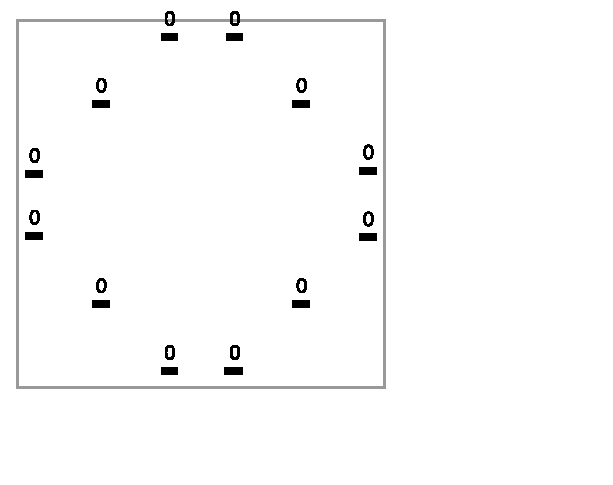
\includegraphics[clip, bb=0bp 20bp 200bp 240bp,scale=0.75]{images/Segment2}\label{segment2}}
    \subfloat[]{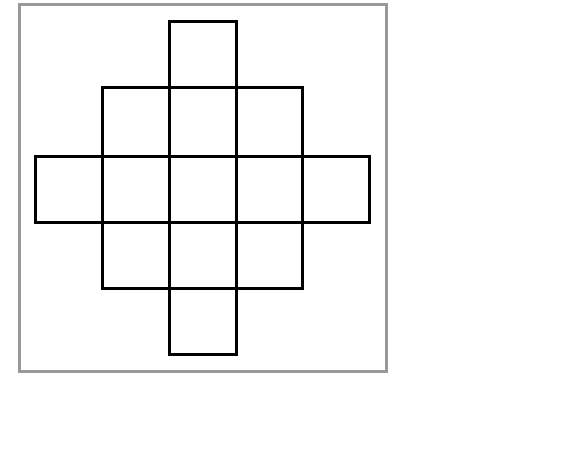
\includegraphics[clip, bb=0bp 20bp 200bp 240bp,scale=0.75]{images/Segment1}\label{segment1}}
    \subfloat[]{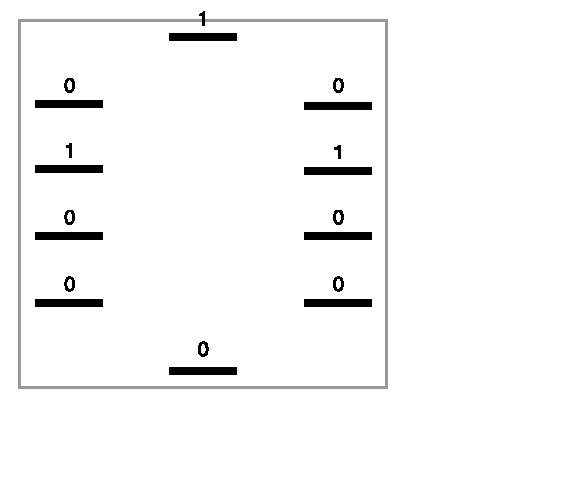
\includegraphics[clip, bb=0bp 20bp 200bp 240bp,scale=0.75]{images/Segment3}\label{segment3}}\\
    \subfloat[]{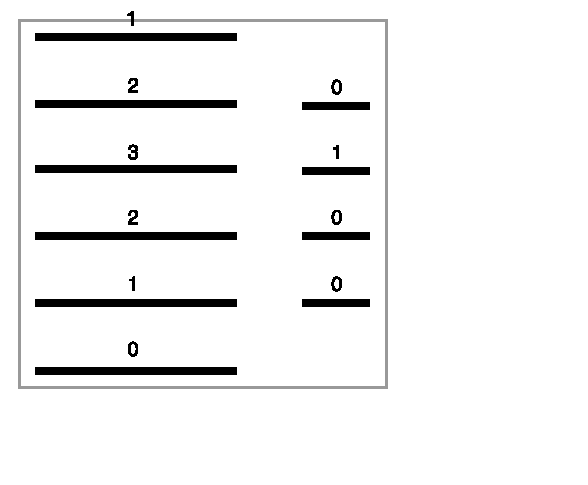
\includegraphics[clip, bb=0bp 20bp 200bp 240bp,scale=0.75]{images/Segment4}\label{segment4}}
    \subfloat[]{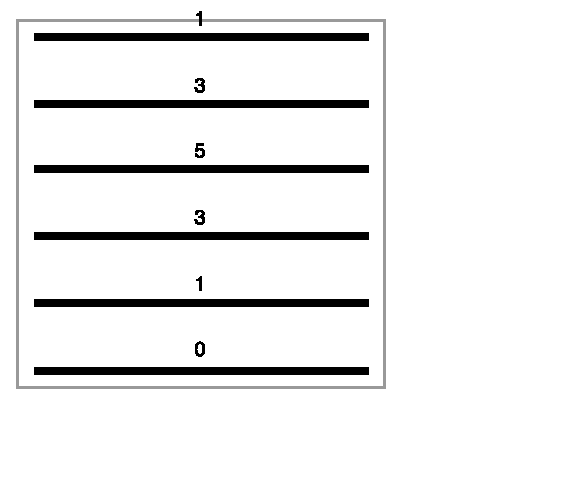
\includegraphics[clip, bb=0bp 20bp 200bp 240bp,scale=0.75]{images/Segment5}\label{segment5}}
    \caption{An execution of the algorithm with $d = 2$.}
    \label{fig:segments}
\end{figure}

%\bibliographystyle{plain}
%\addcontentsline{toc}{section}{\refname}\bibliography{ref}

\end{document}
